\documentclass[oneside,11pt]{memoir}

\usepackage{microtype}
\usepackage{mathptmx}
\usepackage{graphicx}
\usepackage{amsmath}
%\usepackage{color}
\usepackage{xfrac}
\usepackage[group-minimum-digits=3,group-separator={,}]{siunitx}
\usepackage{bigstrut}
\usepackage{hyperref}

\setverbatimfont{\normalfont\ttfamily\small}

\headstyles{bringhurst}
\hypersetup{bookmarksopen,
            bookmarksnumbered,
            colorlinks=true,
            citecolor=red,
            filecolor=red,
            urlcolor=red}

\newsubfloat{figure}
\makepagenote

%-------------------------------------------------------------------------------

\newcommand{\threed}  {3D}
\newcommand{\opengl}  {\textsc{OpenGL}}
\newcommand{\scm}     {\textsc{scm}}
\newcommand{\tiff}    {\textsc{tiff}}
\newcommand{\xml}     {\textsc{xml}}
\newcommand{\panopath}{\textsc{panopath}}
\newcommand{\rgb}     {\textsc{rgb}}
\newcommand{\mb}    {\,\textsc{mb}}
\newcommand{\vram}    {\textsc{vram}}

\newcommand{\B}{\bigstrut[b]}
\newcommand{\T}{\bigstrut[t]}

\newcommand{\Pos}[1]{\phantom{-}{#1}}
\newcommand{\Neg}[1]{        {-}{#1}}

%-------------------------------------------------------------------------------

\begin{document}
\title{Spherical Cube Map TIFF}
\author{Robert Kooima}
\maketitle
\begin{Spacing}{1.1}

% Recursive subdivision
% Effective resolution
% SLERP
%     Demonstrate equivalence of SLERP and recursion?
% Page index mathematical relationships
% Page neighbor relationships

% SCM TIFF
%     Many modes

% Example: WAC global ortho blending
% Example: WAC DTM / LOLA merge

% Appendix: Panoview configuration

\chapter{Spherical Cube Map}

\section{Page Indexing}
The effective sphere map resolution of an \scm\ tree with page size $n$ and depth $d$ is
\[w=n\,2^{d+2}\qquad h=n\,2^{d+1}.\]

The total number of pages in an \scm\ tree of depth $d$ is
\[m=2^{2\,d+3}-2.\]

For reference, the following table shows the effective resolutions and page counts of \scm\ trees with depths down to $7$. Page size $n=512$ is often used for power-of-two source images, and $n=720$ works well for geographic and planetary gridded data.

\begin{center}
\begin{tabular}{r|rr|rr|r}
$d$& $w_{\,512}$& $h_{\,512}$& $w_{\,720}$& $h_{\,720}$& $m$ \B\\\hline
\num{0}&  \num{2048}&  \num{1024}&  \num{2880}&  \num{1440}&     \num{6} \T\\
\num{1}&  \num{4096}&  \num{2048}&  \num{5760}&  \num{2880}&    \num{30} \\
\num{2}&  \num{8192}&  \num{4096}& \num{11520}&  \num{5760}&   \num{126} \\
\num{3}& \num{16384}&  \num{8192}& \num{23040}& \num{11520}&   \num{510} \\
\num{4}& \num{32768}& \num{16384}& \num{46080}& \num{23040}&  \num{2046} \\
\num{5}& \num{65536}& \num{32768}& \num{92160}& \num{46080}&  \num{8190} \\
\num{6}&\num{131072}& \num{65536}&\num{184320}& \num{92160}& \num{32766} \\
\num{7}&\num{262144}&\num{262144}&\num{368640}&\num{184320}&\num{131070} \\
\end{tabular}
\end{center}

Each page is identified by an index giving the page's position in the breadth-first traversal of the page tree. This index provides a natural ordering for stored pages that maximizes locality of reference and ensures that any prefix of a valid \scm\ is also a valid \scm.

The page index uniquely determines each page's size, position, and orientation on the sphere, and the configuration of the first six root pages determines the layout of the data as a whole. This root configuration coincides with the definition of a standard \opengl\ cube map. Pages zero through five map onto the faces of a cube as follows.
\[p_0=+X\quad p_1=-X\quad p_2=+Y\quad p_3=-Y\quad p_4=+Z\quad p_5=-Z\]

Much like the classical binary heap data structure, \scm\ tree indices represent positions in a complete tree, and parent-child relationships follow from straightforward integer arithmetic. If page $p_j$ is the parent of page $p_i$ then
\[j=(i-6)/4.\]

If page $p_i$ is the $k$th child of page $p_j$ then
\[i=6+4\,j+k\]

The child order $k$ of page $p_i$ is
\[k=(i-6)-4\,((i-6)/4).\]

The \scm\ tree level $l$ at which page $p_i$ appears is
\[l=\frac{\lfloor\log_2\,(i+2)\rfloor - 1}{2}\]

When processing and rendering \scm\ data, it is often necessary to know the indices of spatially adjacent pages. This relationship does not emerge readily, and is somewhat more challenging to compute. An implementation, provided in the source, has complexity linear in the distance to the adjacent pages' first common ancestor.

\section{Sample Distribution}

The mapping of \scm\ image data onto the sphere proceeds as follows. For an $n\times n$ raster image applied to the $+Z$ face of the cube, the pixel at row~$r$ and column~$c$ gives a datum at a position on the sphere $(\alpha, \beta)$, where
\[\alpha=90^{\circ}\,\frac{c + \sfrac{1}{2}}{n} - 45^{\circ}\qquad\beta=90^{\circ}\,\frac{r + \sfrac{1}{2}}{n} - 45^{\circ}.\]
which corresponds to the \threed\ vector
\begin{align*}
x& = \phantom{-}\sin\alpha\, \cos\beta\\
y& =         {-}\cos\alpha\, \sin\beta\\
z& = \phantom{-}\cos\alpha\, \cos\beta.
\end{align*}

This vector has length \(\sqrt{\cos^2\,\alpha + \sin^2\,\alpha\,\cos^2\,\beta}\), but when normalization is required, that formulation is not necessarily preferable to the more general \(\sqrt{x^2+y^2+z^2}\).

Vectors within all six root faces are simple $90^\circ$ rotations of this definition, trivially implemented in the form of swizzles and negations. For each face, the vector $(x', y', z')$ toward the sample at row and column $(r, c)$ is defined in terms of $(x, y, z)$ as follows.
\begin{center}
\begin{tabular}{rr|r|r|r|r|r}
    &$\Pos{X}$&$\Neg{X}$&$\Pos{Y}$&$\Neg{Y}$&$\Pos{Z}$&$\Neg{Z}$\\\hline
$x'=$&$\Pos{z}$&$\Neg{z}$&$\Pos{x}$&$\Pos{x}$&$\Pos{x}$&$\Neg{x}$\\
$y'=$&$\Pos{y}$&$\Pos{y}$&$\Pos{z}$&$\Neg{z}$&$\Pos{y}$&$\Pos{y}$\\
$z'=$&$\Neg{x}$&$\Pos{x}$&$\Neg{y}$&$\Pos{y}$&$\Pos{z}$&$\Neg{z}$\\
\end{tabular}
\end{center}

The root face orientations given by this swizzle table do match the definition of a standard \opengl\ cube map, and it is the non-linear mapping from row and column to 3D vector that puts the ``spherical'' in ``spherical cube map.'' While more expensive to compute, this mapping is more amenable to the delivery of high resolution spherical data sets, as it provides a more uniform tesselation of the sphere, and thus a more consistent density of data at every point on its surface.

As depicted by Figure~\ref{fig:cube}, linear cube map samples stretch in the center of the face and compress toward the edges. While all tessellations of the sphere necessarily demonstrate some degree of similar non-uniformity, the spherical cube map, Figure~\ref{fig:scube}, is visibly closer to the impossible ideal. Specifically, the very smallest pixels of a linear cube map, found at the corners, have only $19\%$ of the area of the largest pixels at the cube face centers. In contrast, the smallest pixels of a spherical cube map face, found at the centers of the face edges, have $70\%$ of the area of the largest pixels at the face centers.\pagenote{In an unexpected result, as the resolution of an \scm\ page tends toward infinity, the ratio of the solid angle of a center pixel (the largest pixel) to the solid angle of an edge pixel (the smallest pixel) tends toward exactly $\sqrt{2}/2$.} The corners pixels of an \scm\ are actually \emph{not} the smallest, with $76\%$ the area of the center pixels.

\begin{figure}
  \centering
  \subbottom[Linear cube map]{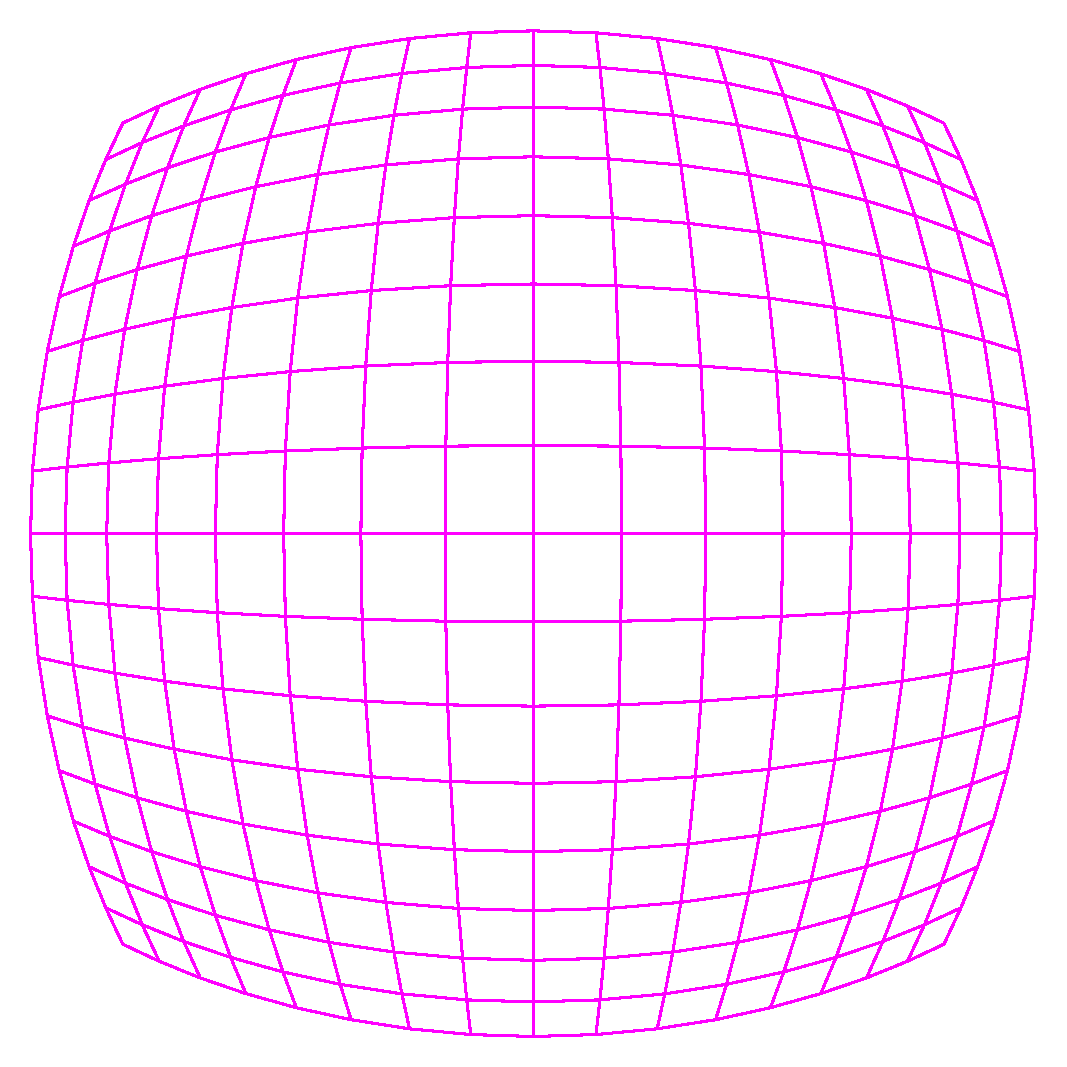
\includegraphics[width=0.3\textwidth]{fig/cube.pdf}\label{fig:cube}}
  \hfil
  \subbottom[Spherical cube map]{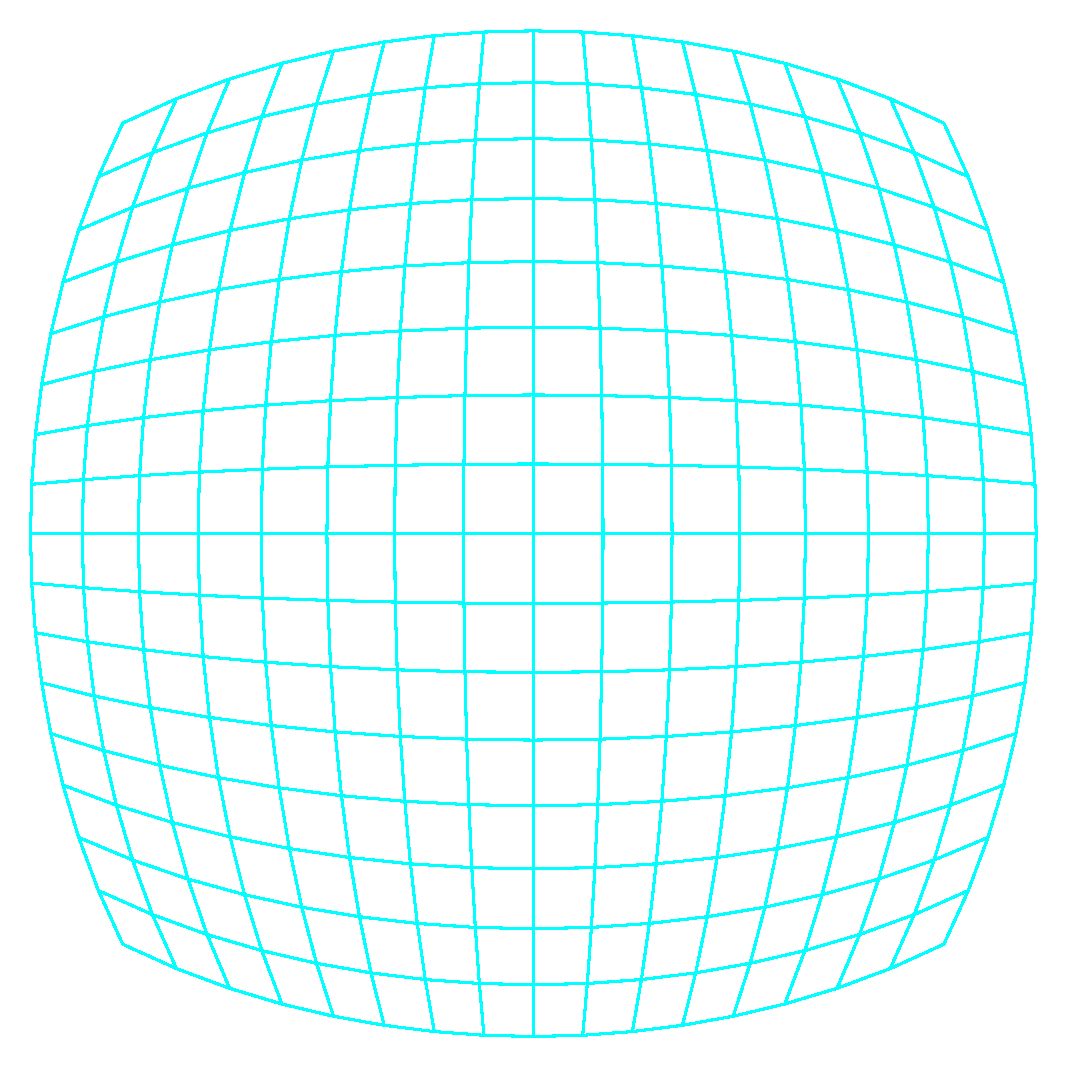
\includegraphics[width=0.3\textwidth]{fig/scube.pdf}\label{fig:scube}}
  \hfil
  \subbottom[Overlaid]{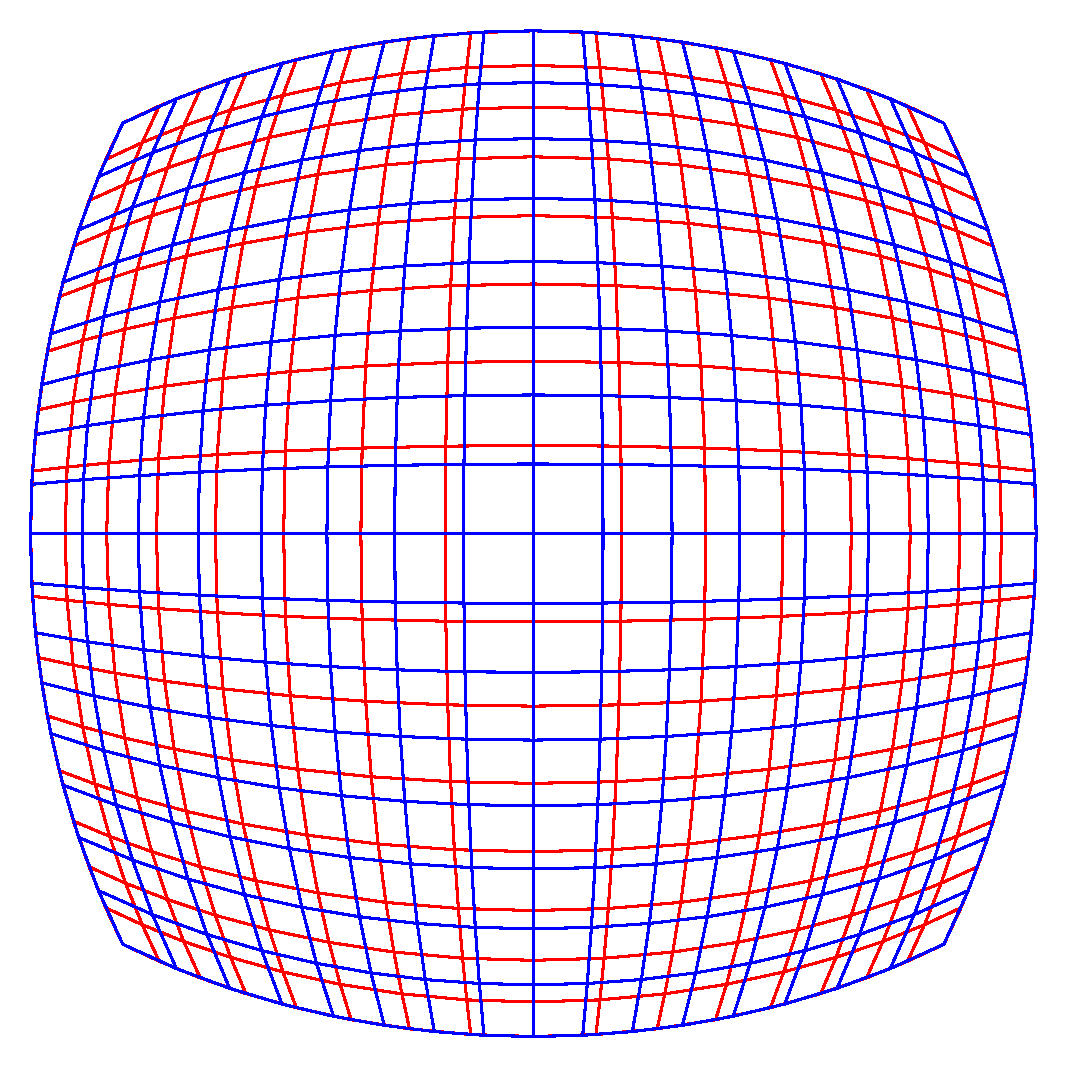
\includegraphics[width=0.3\textwidth]{fig/both.pdf}\label{fig:both}}
  \caption{A comparison of linear and spherical cube map pixel uniformity}
  \label{fig:uniformity}
\end{figure}

Similarly, the shortest edge of the linear cube map is only $47\%$ of the length of the longest, while the shortest edge of the spherical cube map is $70\%$ of the length of the longest. Notably, the pixels along the center row and column of the \scm\ page have equal edge lengths, which means that an \scm\ data set has constant data density along the equator, as well as along four meridians.

% The middle row and column of the scube face have constant edge length

% ratios of longest to shortest sides
% most extreme angles

\chapter{Interactive Display}

\section{Render Library}

The out-of-core panorama renderer is implemented as a small C++ library that may be embedded within any \opengl\ host application. This library has just one system-level configuration parameter:

\panopath\ is a shell environment variable akin to the bash executable path. It lists directories where spherical cube map \tiff\ files may be found. If the application requests that the renderer load a file, but the renderer cannot find that file, then it will search this list of directories. Set this variable in the shell resource file, as need be, separated by colons. For example,

\begin{verbatim}
export PANOPATH=/share/pan:$HOME/data/pan:.
\end{verbatim}

For cluster-driven display systems, try to replicate all panorama image files to local directories on all rendering nodes. This will perform better than data files stored on network shares.

\section{Panorama Definition File}

An example panorama viewer, panoview, is implemented using the Thumb framework. While the previous sections on panorama handling apply to any embedding of the panorama renderer, the following sections describe the configuration and usage specifically of panoview.

For correct display, panoview must understand the parameters of each panoramic image. The panorama definition is an XML file that provides this information.

Like any data file, Thumb must be able to find these panorama definitions. They are appear in the Thumb data hierarchy like any other configuration file. This means they may be placed in a data directory rooted at the current directory, or in the ~/.thumb hierarchy, or in a data hierarchy given by the THUMB\_RO\_DATA environment variable. Panorama definition files need not be stored along side the TIFF files that the reference. It is the PANOPATH environment variable that defines the location of these.

\subsection{Basic Stereo Panorama}

Here is an example of a basic stereo panorama definition, named Blue-Mounds-8.xml.

\begin{verbatim}
<?xml version="1.0"?>
  <panorama channels="2" depth="4" size="512"
      mesh="16" height="0" radius="6"
      vert="glsl/sph-zoomer.vert"
      frag="glsl/sph-render.frag">
  <image channel="0" file="Blue-Mounds-8-L-512-4.tif" />
  <image channel="1" file="Blue-Mounds-8-R-512-4.tif" />
  </panorama>
\end{verbatim}

The file begins with an \xml\ header and contains a single root panorama element with several attributes and one image sub-element for each panorama image.

The channels attribute gives the number view positions. This adapts a panorama definition to a specific display configuration. A desktop display will have one channel, a CAVE will have two, and a multi-view lenticular may have many more.

The size and depth attributes give the size of each page in the panorama image files and the depth of their page hierarchies. Note that the values coincide with the image parameters given by the file names. Other values are allowed, and may enable quality-speed tradeoffs.

The mesh attribute determines the tesselation of the geometry mesh used to render each page of data. The example value, 16, indicates that each page of the sphere will be rendered using a $16\times 16$ grid of polygons. There is little reason to change this.

The radius attribute determines the radius of the spherical proxy geometry used to render the panorama. The height attribute determines the placement of the proxy geometry in the scene, and should match the height of the camera at the time the panorama was captured. These values are given in meters, and are mostly significant in VR display environments. The default radius is 6 meters, and the default height is 0 meters.

The vert and frag attributes give the vertex and fragment programs to be used by the renderer, named relative to the root of the Thumb data hierarchy. These will remain the same for most panorama definitions.The zoomer; vertex program must be specified for zoomable panoramas. The render fragment program is used for static panoramas such as this one.

\subsection{Multi-image Panorama}

The following example, Taliesin-Path, is more complex. It defines several images for each channel. This will behave as a circular list of images, and the renderer will interpolate between them in order, following an internal “playback head.”

\begin{verbatim}
<?xml version="1.0"?>
  <panorama channels="2" depth="3" size="512"
      vert="glsl/sph-zoomer.vert"
      frag="glsl/sph-blend.frag">
  <image channel="0" file="Taliesin-Path-A-L-512-3.tif" />
  <image channel="1" file="Taliesin-Path-A-R-512-3.tif" />
  <image channel="0" file="Taliesin-Path-B-L-512-3.tif" />
  <image channel="1" file="Taliesin-Path-B-R-512-3.tif" />
  <image channel="0" file="Taliesin-Path-C-L-512-3.tif" />
  <image channel="1" file="Taliesin-Path-C-R-512-3.tif" />
  <image channel="0" file="Taliesin-Path-D-L-512-3.tif" />
  <image channel="1" file="Taliesin-Path-D-R-512-3.tif" />
  <image channel="0" file="Taliesin-Path-E-L-512-3.tif" />
  <image channel="1" file="Taliesin-Path-E-R-512-3.tif" />
  <image channel="0" file="Taliesin-Path-F-L-512-3.tif" />
  <image channel="1" file="Taliesin-Path-F-R-512-3.tif" />
  <image channel="0" file="Taliesin-Path-G-L-512-3.tif" />
  <image channel="1" file="Taliesin-Path-G-R-512-3.tif" />
  <image channel="0" file="Taliesin-Path-H-L-512-3.tif" />
  <image channel="1" file="Taliesin-Path-H-R-512-3.tif" />
  </panorama>
\end{verbatim}

Note that the frag attribute of the panorama element specifies the blend fragment program. This program performs the interpolation. Non-interpolating panoramas should use the \texttt{sph-render.vert} program, as \texttt{sph-blend.vert} doubles the texture access load of the renderer.

\section{Panoview Usage}

Panoview is configured and run like any other Thumb application. The following keyboard commands are defined.

\begin{itemize}
\item[F1] Toggle the panoview file selection dialog. This dialog allows the user to navigate the Thumb data hierarchy and select a panorama definition for viewing.

\item[F2] Toggle the cache visualization overlay. This allows the set of all resident pages to be viewed in thumbnail.

\item[F3] Toggle the page coloration debug view. This feature recolors each incoming page to indicate its depth in the page tree.

\item[F4] Toggle automatic zoom centering. This option controls whether the center of the zoom is static or dynamic.
\end{itemize}

In addition, there is one option in the Thumb configuration file conf.xml that impacts the behavior and performance of the panorama renderer.

\begin{verbatim}
<option name="panoview_cache_size">128</option>
\end{verbatim}

This option selects the maximum number of pages that may be loaded at any given moment. A $512\times 512$ page of \rgb\ data consumes 1\mb\ of \vram\, and this cache size option should be set accordingly. A larger value gives better performance, but too large a value will result in catastrophically bad performance.

\section{Troubleshooting}

This is a list of issues to be aware of, should trouble arise.

\begin{itemize}
\item If the panorama definition \xml\ files are not visible in the panoview file loader, then be sure they are located within the Thumb data hierarchy, or add their location to the Thumb data hierarchy by including the path in the \textsc{thumb\_ro\_path} environment variable.

\item If the panorama definition loads but does not display an image, be sure the path to the spherical cube map \tiff\ files appears in the \panopath\ environment variable.

\item If a multi-image panorama jumps from one panorama to the next instead of fading, be sure the blend fragment program is referenced by the definition.

\item In general, be sure that the depth and size attributes of the panorama definition match the input files.

\item If performance is sluggish, be sure that panorama image files are not being accessed from a network share.
\end{itemize}

\printpagenotes
\end{Spacing}
\end{document}
